%\documentclass[11pt]{amsart}
\documentclass[12pt]{article}
\usepackage[top=0.6in,bottom=.5in,left=.8in,right=.8in]{geometry}
\usepackage{geometry}                % See geometry.pdf to learn the layout options. There are lots.
\geometry{letterpaper}                   % ... or a4paper or a5paper or ... 
%\geometry{landscape}                % Activate for for rotated page geometry
%\usepackage[parfill]{parskip}    % Activate to begin paragraphs with an empty line rather than an indent
\usepackage{graphicx}
\usepackage{amsmath}
\usepackage{amssymb}
\usepackage{epstopdf}
\usepackage{tikz}
\usetikzlibrary{arrows}
\usepackage{algpseudocode}
\DeclareGraphicsRule{.tif}{png}{.png}{`convert #1 `dirname #1`/`basename #1 .tif`.png}
\linespread{1.5}

\title{Hardware RSA Accelerator}
\author{Group 3: Ariel Anders, Timur Balbekov, Neil Forrester}
%\date{}                                           % Activate to display a given date or no date

\begin{document}

\maketitle

\section{Overview}
Our project proposal is implementing the RSA cryptographic algorithm in Bluespec.
The benefits of doing this in hardware are higher performance, reduced power usage and size, and cost.
Having reusable IP that implements RSA would allow a device manufacturer to skip the inclusion
of a processor in a device that requires secure communications, but otherwise wouldn't need one. 

An example application of our preliminary proposal could be an intelligence agencies' covert listening device
with the added ability of secure communication through RSA protocol.
Specialized hardware is useful here because the device needs to be small,
without excessive power consumption, and the ability to run for long periods of time. 

Alternatively, suppose you were designing a high performance router to create a secure VPN between remote sites,
so that it appears that all the computers at all sites are on the local network.
Keeping latency as low as possible, and throughput as high as possible, would be vital.
Hardware support for Public Key Cryptography, such as RSA,
could play an essential component in developing this router.

The main challenges we foresee in implementing RSA in Bluespec are creating a multi-precision arithmetic library
with support for modulo, exponentiation, and multiplication.
Once those problems are solved, the only remaining issue is writing a sensible interface.

\section{Implementation}

\section{MicroArchitecture}

\subsection{Naive Modular Multiply}
The naive modular multiply does not use any of the specialized algorithms
specifically tuned for hardware implementations.
The overview of this module is pictured in Figure \ref{fig-naive}.

\begin{figure}
  \begin{centering}
    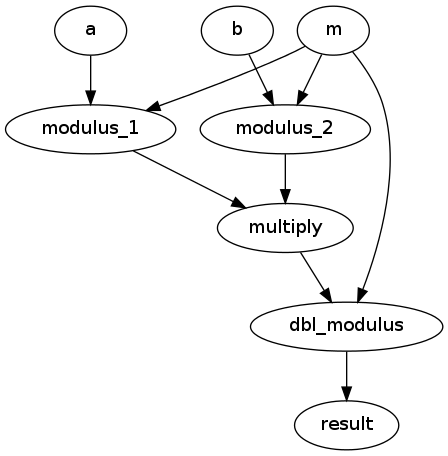
\includegraphics[width=0.4\textwidth]{modMultGraph.png}
    \caption{Naive Modular Multiplication}
    \label{fig-naive}
  \end{centering}
\end{figure}

One particular bottleneck of this implementation is the 2048 bit width result from the multiply block
resulting in a very long implementation for {\tt dbl\_modulus}.


\section{Algorithms}
All of our high-level RSA modules will be built around a single module that does modular exponentiation.
Unless some unforeseen detail necessitates a change, this module will employ the Right-to-left binary algorithm
(which we believe will be a good compromise between speed, memory usage, and complexity).
The goal of the algorithm is to calculate $b^e \bmod m$ for very large values of $b$, $e$, and $m$.
If the bits of $e$ are $e_1, e_2 \dots e_n$:
\begin{equation}
e = \sum_{i = 0}^{n} e_i 2^i
\end{equation}
then:
\begin{equation}
b^e = \prod_{i = 0}^{n} e_i b^{(2^i)}
\end{equation}
and since:
\begin{equation}
a * b \bmod m = (a \bmod m) * (b \bmod m) \bmod m
\end{equation}
then every intermediate result can be taken modulo $m$ to keep the size of intermediate results manageable.
Therefore, the following algorithm will compute $b^e \bmod m$ in a reasonable amount of time and memory:
\begin{algorithmic}
\While{$e > 0$}
	\If{$e \bmod 2 = 1$}
		\State $c \gets c * b \bmod m$
	\EndIf
	\State $b \gets b * b \bmod m$
	\State $e \gets \lfloor e / 2 \rfloor$
\EndWhile
\end{algorithmic}
This very naturally suggests a circular pipeline in hardware.
If parallelism is desired, then multiple circular pipelines may be put in parallel,
with some logic at the front and back to manage handing out jobs to different circular pipelines,
and collecting the results.

The only remaining problem is performing multiplication, modulo, and bit shifting
on integers that are thousands of bits long.
If it turns out to be practical to simply instantiate registers of types like {\tt Int\#(4096)},
and perform combinational operations on them by writing {\tt a~*~b}, {\tt a~\%~m}, and {\tt a~>>~1},
then that's fantastic.
We will investigate this possibility.

Unfortunately, we suspect that this may consume a tremendous amount of area,
introduce long combinational delays, or cause other undesirable behavior.
If so, then it will be necessary to handle large integers another way.
We propose storing integers in BRAM, as a series of bytes.
We will then be free to implement algorithms for arithmetic operations
which operate on only a small number of bits at a time. In particular, we can 
explore the redundant interleaved modular exponentiation algorithm, which does
not perform full length (1024x1024) multiplication. 

\section{Verification}
To verify the functionality of the RSA module, we will initially separately 
compare the results of the encryption and decryption blocks to the results
of a software implementation. The two private keys for encryption and
decryption modules will be burned into the hardware. A SceMi testbench will
push a message to the encryption block, along with an enable signal, message,
and public key of the software testbench. The module will generate an encrypted message,
and the software testbench will use its private key to decrypt and verify the 
correctness of the encrypted message.

For decryption, the process is reversed: the testbench will pass in an 
encrypted message instead of plaintext, and the decryption module will use
the private key of the software testbench to decrypt the message. The testbench
will verify the plaintext for correctness.

After individual testing of the blocks, we will add support for confirming the signature
(authenticity checking) of the transmitted message. The testbench will hash the plaintext
message before encryption, and use the private key as the exponent (as if it was decrypting
the hash). The hardware decryption module will use the testbench's public key as the exponent
(as during encryption) to retrieve the hash as calculated by the sender. If the hash of the
decrypted message matches the original hash, then the message is genuine. The testbench
will purposefully tamper with the encrypted message to prove the correctness of the 
signature detection mechanism. 

To prove correctness to the instructors, a simple testbench will feed plaintext into an
encryption-decryption block pair (connected via a FIFO).

\end{document}  
